% ----------------------------------------------------------
\chapter{Fundamentação teórica}\label{cap:desenvolvimento}
% ----------------------------------------------------------
Neste capitulo apresenta-se uma visão de como funcionam os algoritmos e estruturas de dados base para o desenvolvimento
de algoritmos para renderização em janela acesso rápido para estruturas geométricas.
Sao os algoritmos e estruturas de dados base para a construção de um controle de janela para acesso rapido de poligonos
em janela.



% ----------------------------------------------------------
\section{Arvores KD}
% ----------------------------------------------------------

Uma Arvore KD é uma arvore binaria onde cada folha é um ponto \textit{k-dimensional}.
E cada nodo não-folha é um corte do espaço, representando implicitamente um hiperplano.
Pontos a esquerda desse hiperplano estão na subárvore da esquerda, e respectivamente para o lado direito.
Cada nodo é associado com uma das \textit{k dimensões}. Então, a citar um exemplo, se dado nodo divide o eixo
x, a subárvore a esquerda contem os pontos com o eixo x menor que o ponto de corte.

\begin{figure}[htb]
    \caption{\label{fig:Fig_1}Arvore k\textit{dimensional} - 3D}
    \begin{center}
        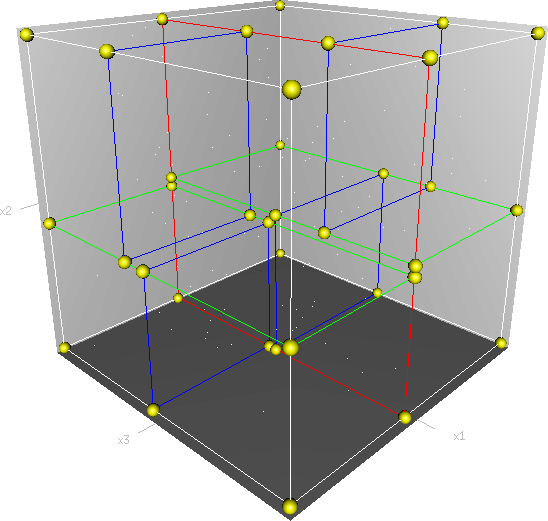
\includegraphics[width=\linewidth/2]{images/3dtree.png}
    \end{center}
    \fonte{GPL}
\end{figure}

\subsection{Construção da Árvore}
A termos didáticos segue a construção da arvore KD de 2 dimensões.
Seja \textit{P} o conjunto de \textit{n} pontos em um plano.

Uma busca de alcance 2-dimensional em \textit{P} é uma busca de quais pontos da busca estão
entre o retângulo de busca \([x,x'] X [y,y']\). Um ponto \textit{p}\(:= (p_x, p_y)\) está dentro do retângulo
de busca se e somente se:

\[
    p_x \in [x, x']  \text{ e } p_y \in [y,y']
\].

Podemos dizer que uma busca 2-dimensional é composta de duas sub-buscas 1-dimensional, uma no
eixo \(x\)-coordenada de um dos pontos e um na \(y\)-coordenada.

\begin{figure}[htb]
    \caption{\label{fig:Fig_2}Busca em alcance \textit{dimensional} - 2D}
    \begin{center}
        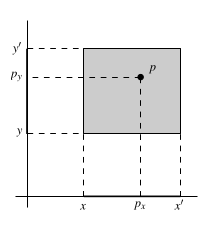
\includegraphics{images/search_range.png}
    \end{center}
    \fonte{Computational Geometry}
\end{figure}

Na construção de uma arvore para 2 dimensões, cada ponto tem uma \(x\)-coordenada e uma
\(y\)-coordenada.
Seguimos então escolhendo um eixo inicial e salvando o valor de corte deste eixo que divide
os pontos deste eixo em dois conjuntos, e no próximo nível da arvore, alterna-se o eixo e repete-se
o processo recursivamente.


\begin{figure}[htb]
    \caption{\label{fig:Fig_3} Arvore 2D}
    \begin{center}
        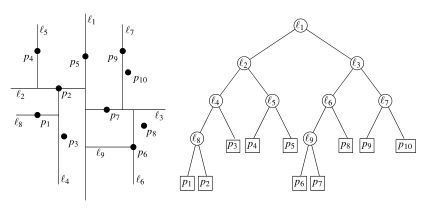
\includegraphics{images/kd_tree1.png}
    \end{center}
\end{figure}

Na raiz ordena-se todos os pontos e divide o conjunto de pontos \(P\) com uma linha vertical
\(l\) que divide os pontos pelo eixo \(x\). Guarda-se o valor de \(x_v\) no nodo e alterna-se o
eixo.
Agora, recursivamente repete o processo para os dois subconjuntos de pontos:
Ordena-se os pontos pelo eixo \(y\) e divide o conjunto e encontra-se a reta horizontal que
subdivide os pontos e guarda no nodo do valor de corte \(y\).
A condição de parada é até quando o conjunto de pontos restantes contiver apenas um ponto.
Este sendo então o nodo folha.


\begin{algorithm}
    \caption{ConstroiArvoreKD($Pontos, profundidade$)}
    \begin{algorithmic}
        \IF{P contem apenas um ponto}
        \RETURN $P$
        \ELSE
        \STATE{
            \IF{$profundidade$ é par}
            \STATE{
                Divide P em dois subconjuntos com um linha vertical $l$ pela mediana da $x-coordenada$
                dos pontos em P. Seja $P_1$ o conjunto dos pontos à esquerda de $l$ e seja
                $P_2$ o conjunto de pontos à direita de $l$.
            }
            \ELSE
            \STATE{
                Divide P em dois subconjuntos com um linha horizontal $l$ pela mediana da $y-coordenada$
                dos pontos em P. Seja $P_1$ o conjunto dos pontos acima de $l$ e seja
                $P_2$ o conjunto de pontos à abaixo de $l$.
            }
            \ENDIF
        }
        \ENDIF

        \STATE $v_{esquerda} \leftarrow $ ConstroiArvoreKD($P_1, profundidade+1$)
        \STATE $v_{direita} \leftarrow $ ConstroiArvoreKD($P_2, profundidade+1$)
        Cria um nodo $v$ guardando $l$ e fazendo $v_esquerda$ o nodo da esquerda
        de $v$ e fazendo $v_direita$ nodo da direita de $v$.

        \RETURN $v$
    \end{algorithmic}
\end{algorithm}

\subsection{Busca com alcance}

Agora retomamos para o algoritmo de busca. Podemos imaginar que os pontos na subárvore à esquerda
da raiz, estão limitados à direita pela reta com o eixo \(x\) com valor de \(x \leq l_1\).
Enquanto os pontos na subárvore à direita do nodo \(l_1\) estão limitados com o eixo \(x > l_1\).

A exemplo: o nodo \(l_4\), a região correspondente de \(l_4\) é limitada à esquerda de
\(l_1\) e abaixo de \(y\) do nodo \(l_2\).

\begin{figure}[htb]
    \caption{\label{fig:Fig_4} Área respectiva de um nodo}
    \begin{center}
        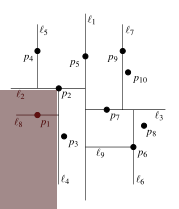
\includegraphics{images/kd_tree2.png}
    \end{center}
\end{figure}

Denotaremos esta área de um nodo \(v\) como \(regiao(v)\). A região da raiz é simplesmente
(no caso de uma arvore 2D) o plano inteiro.
Portanto o algoritmo buscará a subárvore de \(v\) somente se o retângulo de busca intersectar
a \(regiao(v)\).
O algoritmo de busca funciona descendo a arvore mas visitando somente os nodos que a
\(regiao(v)\) intersecta o retângulo da busca. Quando uma \(regiao(v)\) esta contido no
retângulo de busca retornamos todos os pontos na subárvore.
Quando chegarmos nos nodos folhas temos de checar se o nodo esta dentro da busca, se tiver,
retorna-o.

Segue o algoritmo que recebe como parâmetros a raiz da arvore-KD e o retângulo de busca \(R\).
Usa-se uma chamada \(RetornaSubarvore(v)\) que atravessa a arvore de nodo \(v\) e retorna
todos os pontos nas suas folhas. Segue como notação \(fe(v)\) sendo o filho da esquerda e
\(fd(v)\) o filho da direita do nodo \(v\).


\begin{algorithm}
    \caption{BuscaEmArvoreKD($v, Busca$)}
    \begin{algorithmic}
        \IF{v é folha}
        \STATE{Retorna o ponto de $v$ se estiver dentro da $Busca$}
        \ELSE
        \STATE{
            \IF{$regiao(fe(v))$ está contido na $Busca$}
            \STATE{$RetornaSubarvore(v)$}
            \ELSE
            \STATE{
                \IF{$regiao(fe(v))$ intersecta $Busca$}
                \STATE{
                    $BuscaEmArvoreKD(fe(v), Busca)$
                }
                \ENDIF
            }
            \ENDIF

            \IF{$regiao(fd(v))$ está contido na $Busca$}
            \STATE{$RetornaSubarvore(v)$}
            \ELSE
            \STATE{
                \IF{$regiao(fd(v))$ intersecta $Busca$}
                \STATE{
                    $BuscaEmArvoreKD(fd(v), Busca)$
                }
                \ENDIF
            }
            \ENDIF
        }
        \ENDIF
    \end{algorithmic}
\end{algorithm}

A principal comparação realizada é checar se a área de \(Busca\) intersecta a região
de um nodo \(v\). Para isso precisamos computar \(regiao(v)\) para todos os nodos \(v\)
durante a fase de construção da arvore.
Uma alternativa é manter a região salva nas chamadas recursivas usando as linhas guardadas
nos nodos internos. Por exemplo a região correspondente ao filho esquerda de um nodo
\(v\) em uma profundidade par (no exemplo 2D, analisamos no eixo \(x\)) pode ser calculado com:
\[
    regiao(fe(v)) = regiao(v) \cap l(v)^{esquerda}
\],
onde \(l(v)\) é a linha que divide o eixo salvo em \(v\), e \(l(v)^{esquerda}\) é a metade
esquerda do plano.


% ----------------------------------------------------------
\section{Arvore de Intervalos}
% ----------------------------------------------------------

% No que diz respeito à estrutura do trabalho, recomenda-se que:
% \begin{alineas}
% 	\item o texto deve ser justificado, digitado em cor preta, podendo utilizar outras cores somente para as ilustrações;
% 	\item utilizar papel branco ou reciclado para impressão;
% 	\item os elementos pré-textuais devem iniciar no anverso da folha, com exceção da ficha catalográfica ou ficha de identificação da obra;
% 	\item os elementos textuais e pós-textuais devem ser digitados no anverso e verso das folhas, quando o trabalho for impresso. As seções primárias devem começar sempre em páginas ímpares, quando o trabalho for impresso. Deixar um espaço entre o título da seção/subseção e o texto e entre o texto e o título da subseção.
% \end{alineas}

% No \autoref{qua:Quadro_1} estão as especificações para a formatação do texto.

% \begin{quadro}[htb]
% 	\centering
% 	\caption{\label{qua:Quadro_1}Formatação do texto.}
% 	\begin{tabular}{|l|p{11cm}|}
% 		\hline
% 		\textbf{Formato do papel} & A4.                                                                                                                                                                                                                                                                                                                                                                                                                                 \\ \hline
% 		\textbf{Impressão}        & A norma recomenda que caso seja necessário imprimir, deve-se utilizar a frente e o verso da página.                                                                                                                                                                                                                                                                                                                                 \\ \hline
% 		\textbf{Margens}          & Superior: 3, Inferior: 2, Interna: 3 e Externa: 2. Usar margens espelhadas quando o  trabalho for impresso.                                                                                                                                                                                                                                                                                                                         \\ \hline
% 		\textbf{Paginação}        & As páginas dos elementos pré-textuais devem ser contadas, mas não numeradas. Para trabalhos digitados somente no anverso, a numeração das páginas deve constar no canto superior direito da página, a 2 cm da borda, figurando a partir da primeira folha da  parte textual. Para trabalhos digitados no anverso e no verso, a numeração deve constar no canto superior direito, no anverso, e no canto superior esquerdo no verso. \\ \hline
% 		\textbf{Espaçamento}      & O texto deve ser redigido com espaçamento entre linhas 1,5, excetuando-se as citações de mais de três linhas, notas de rodapé, referências, legendas das ilustrações e das tabelas, natureza (tipo do trabalho, objetivo, nome da instituição a que é submetido e área de concentração), que devem ser digitados em espaço simples, com fonte menor. As referências devem ser separadas entre si por um espaço simples em branco.   \\ \hline
% 		\textbf{Paginação}        & A contagem inicia na folha de rosto, mas se insere o número da página na introdução até o final do trabalho.                                                                                                                                                                                                                                                                                                                        \\ \hline
% 		\textbf{Fontes sugeridas} & Arial ou Times New Roman.                                                                                                                                                                                                                                                                                                                                                                                                           \\ \hline
% 		\textbf{Tamanho da fonte} & \textbf{Fonte tamanho 12 para o texto}, incluindo os títulos das seções e subseções. As citações com mais de três linhas, notas de rodapé, paginação, dados internacionais de catalogação, legendas e fontes das ilustrações e das tabelas devem ser de tamanho menor. Adotamos, neste \textit{template} \textbf{fonte tamanho 10}.                                                                                                 \\ \hline
% 		\textbf{Nota de rodapé}   & Devem ser digitadas dentro da margem, ficando separadas por um espaço simples por entre as linhas e por filete de 5 cm a partir da margem esquerda. A partir da segunda linha, devem ser alinhadas embaixo da primeira letra da primeira palavra da primeira linha.                                                                                                                                                                 \\ \hline
% 	\end{tabular}
% 	\fonte{\textcite{NBR14724:2011}.}
% \end{quadro}

% % ----------------------------------------------------------
% \subsubsection{As ilustrações}
% % ----------------------------------------------------------

% Independentemente do tipo de ilustração (quadro, desenho, figura, fotografia, mapa, entre outros), a sua identificação aparece na parte superior, precedida da palavra designativa.

% \begin{citacao}
% 	Após a ilustração, na parte inferior, indicar a fonte consultada (elemento obrigatório, mesmo que seja produção do próprio autor), legenda, notas e outras informações necessárias à sua compreensão (se houver). A ilustração deve ser citada no texto e inserida o mais próximo possível do texto a que se refere. \cite[p. 11]{NBR14724:2011}.
% \end{citacao}

% % ----------------------------------------------------------
% \subsubsection{Equações e fórmulas}
% % ----------------------------------------------------------

% As equações e fórmulas devem ser destacadas no texto para facilitar a leitura.  Para numerá-las, usar algarismos arábicos entre parênteses e alinhados à direita. Pode-se adotar uma entrelinha maior do que a usada no texto \cite{NBR14724:2011}.

% Exemplos, \autoref{eq:Eq_1} e \autoref{eq:Eq_2}.

% \begin{equation}\label{eq:Eq_1}
% 	\gls{C} = 2 \gls{pi} \gls{r}
% \end{equation}

% \begin{equation}\label{eq:Eq_2}
% 	\gls{A} = \gls{pi} \gls{r}^2
% \end{equation}
% ----------------------------------------------------------
\section{Arvore de Segmentos}
% ----------------------------------------------------------

% De acordo com \textcite{ibge1993}, tabela é uma forma não discursiva de apresentar informações em que os números representam a informação central. Ver \autoref{tab:Tab_1}.

% \begin{table}[htb]
% 	\ABNTEXfontereduzida
% 	\caption{\label{tab:Tab_1}Médias concentrações urbanas 2010-2011.}
% 	\begin{tabular}{@{}p{3.0cm}p{1.5cm}p{2cm}p{2.5cm}p{2.5cm}p{2.5cm}@{}}
% 		\toprule
% 		\textbf{Média concentração urbana} & \multicolumn{2}{l}{\textbf{População}} & \textbf{Produto Interno Bruto – PIB (bilhões R\$)} & \textbf{Número de empresas} & \textbf{Número de unidades locais}         \\ \midrule
% 		\textbf{Nome}                      & \textbf{Total}                         & \textbf{No Brasil}                                 &                             &                                    &       \\
% 		Ji-Paraná (RO)                     & 116 610                                & 116 610                                            & 1,686                       & 2 734                              & 3 082 \\
% 		Parintins (AM)                     & 102 033                                & 102 033                                            & 0,675                       & 634                                & 683   \\
% 		Boa Vista (RR)                     & 298 215                                & 298 215                                            & 4,823                       & 4 852                              & 5 187 \\
% 		Bragança (PA)                      & 113 227                                & 113 227                                            & 0,452                       & 654                                & 686   \\ \bottomrule
% 	\end{tabular}
% 	\fonte{\textcite{ibge2016}.}
% \end{table}